\documentclass[../Cours.tex]{subfiles}

\begin{document}
\clearpage
\thispagestyle{empty}
\color{black}

\titreDScorrection

\begin{questions}
\EXERCICE{}

\question Dans le cas où la voiture roule à \qty{20}{\metre\per\second}, pour un temps de réaction de 1 seconde, la distance de réaction est de 20 mètres.

\question On applique la formule :
$$D_f = \frac{v^2}{2 \times g \times a} = \frac{20^2}{2 \times 10 \times 0,6} = \qty{33,3}{\metre} $$

La distance de freinage est donc de \qty{33,3}{\metre}.

\question On additionne les résultats des deux questions précédentes : $20 + 33,3 = \qty{53,3}{\metre}$.

\EXERCICE{}

Sur la figure 0, il y a 1 carré.\\
Sur la figure 1, il y a 4 carrés.\\
Sur la figure 2, il y a 7 carrés.\\

À chaque fois que l'on passe à la figure suivante, on augmente le nombre de carrés de 3.

Sur la figure 3, il y a 1 + 3 + 3 + 3 = 7 carrés. (on ajoute 3 fois le 3)\\
Sur la figure 10, il y a 1 + 3 + 3 + ... + 3 = 31 carrés. (on ajoute 10 fois le 3)\\
Sur la figure 100, il y a 1 + 3 + 3 + ... + 3 = 301 carrés. (on ajoute 100 fois le 3)\\
Sur la figure $n$, il y a 1 + 3 + 3 + ... + 3 = $3n+1$ carrés. (on ajoute $n$ fois le 3)

\EXERCICE{}

Le volume d'une boule de glace est égal à $\frac{4}{3} \times \pi \times r^3$, soit $\frac{4}{3} \times \pi \times 5^3 = \qty{523.6}{cm\cubed}$. Le restaurant a 1 000 litres de glace à la vanille et 500 litres de glace au chocolat, soit 1 500 litres de glace en tout. Chaque litre de glace contient \qty{1000}{\centi\metre\cubed}, donc le restaurant a \qty{1500000}{\centi\metre\cubed} de glace. Chaque dame blanche contient 3 boules de glace, soit $3 \times \qty{523,6}{\centi\metre} = \qty{1570}{\centi\metre\cubed}$ de glace. Le restaurant a donc $1 500 000 \div 1570,8 = 952$ dames blanches.

\clearpage
\EXERCICETITRE{4}{THALÈS}

\begin{center}
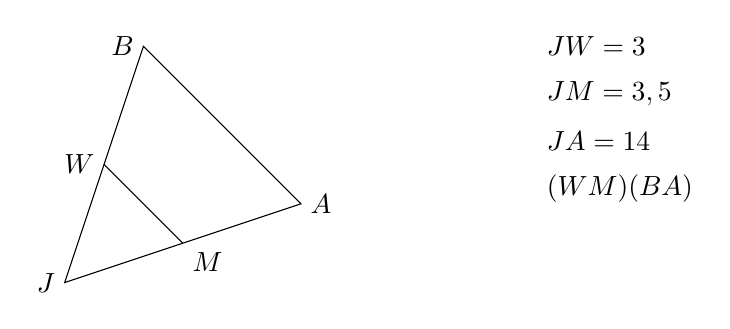
\begin{tikzpicture}
    \draw (0,0) node[left]{$J$} -- (1,3) node[left]{$B$} -- (3,1) node[right]{$A$} -- cycle;
    \draw (0.5,1.5) node[left]{$W$} -- (1.5,0.5) node[below right]{$M$};
    \node[anchor=west] at (6,3) {$JW = 3$};
    \node[anchor=west] at (6,2.4) {$JM = 3,5$};
    \node[anchor=west] at (6,1.8) {$JA = 14$};
    \node[anchor=west] at (6,1.2) {$(WM) \paral (BA)$};
\end{tikzpicture}
\end{center}

\question Déterminons $JB$

\begin{enumerate}
    \item 
    \begin{itemize}
        \item Les points J, W, B sont alignés.
        \item Les points J, M, A sont alignés.
        \item $(WM) \paral (BA)$
    \end{itemize}
    \item D'après le théorème de Thalès :
    \item $\dfrac{JB}{JW} = \dfrac{JA}{JM} = \dfrac{BA}{WM}$
    \item $\dfrac{JB}{3} = \dfrac{14}{\num{3.5}} = \dfrac{BA}{WM}$

    Par un produit en croix, $JB = \dfrac{3 \times 14}{3,5} = 12$
\end{enumerate}

\EXERCICETITRE{5}{THALÈS ET PYTHAGORE}

$ABR$ est un triangle rectangle $B$, tel que $AB = 17$ et $BR = 19$. \\
Placer $I$ sur $[AB]$ tel que $AI=3$. \\
On trace une droite $(d)$ perpendiculaire à $(AB)$ passant par $I$, coupant $(AR)$ en $J$.

Faisons un schéma : 

\begin{center}
    \begin{tikzpicture}[scale=0.3]
        \draw (0,0)--(17,0)--(17,19)--cycle;
        \draw (3,-3) -- (3,10);
        \draw[fill=black] (17,0) rectangle (16.5,0.5);
        \draw[fill=black] (3,0) rectangle (2.5,0.5);
        \node[right] at (3,9) {$(d)$};
        \node[left] at (0,0) {A};
        \node[right] at (17,0) {B};
        \node[right] at (17,19) {R};
        \node[above right] at (3,0) {I};
        \node[left] at (3,4) {J};
        \node[rouge,below] at (1.5,-0.5) {3};
        \draw[latex-latex,rouge] (0,-0.5) -- (3,-0.5);
        \node[vert,below] at (8.5,-2.5) {17};
        \draw[latex-latex,vert] (0,-2.5) -- (17,-2.5);
        \node[bleu,right] at (19,9.5) {19};
        \draw[latex-latex,bleu] (19,0) -- (19,19);
    \end{tikzpicture}
\end{center}

\clearpage
\question Calculons $AR$

On cherche à calculer $AR$, or dans le triangle rectangle $ABR$ on connaît déjà deux longueurs : $AB$ et $BR$. On va donc ici utiliser le théorème de Pythagore.

\begin{enumerate}
    \item Le triangle $ABR$ est rectangle en $B$. L'hypoténuse est $[AR]$.
    \item D'après le théorème de Pythagore :
    \item $$AR^2 = AB^2+BR^2$$
    \item \begin{align*}
        AR^2 &= 17^2 + 19^2 \\
        &= 289 + 361 \\
        &= 650\\
        AR &= \sqrt{650} \\
        &\approx 25,5 
    \end{align*}
\end{enumerate}

\question Calculons $IJ$

On cherche à calculer $IJ$. Dans le triangle rectangle $AIJ$, on ne connaît que la longueur $AI$. C'est insuffisant. On va donc utiliser le théorème de Thalès.

\begin{enumerate}
    \item 
    \begin{itemize}
        \item Les points A, J et R sont alignés.
        \item Les points A, I et B sont alignés.
        \item $(IJ) \paral (BR)$ (car $(IJ) \perp (AB)$ et $(BR) \perp (AB)$)
    \end{itemize}
    \item D'après le théorème de Thalès :
    \item $$\dfrac{AR}{AJ} = \dfrac{AB}{AI} = \dfrac{RB}{JI}$$
    \item $$\dfrac{25,5}{AJ} = \dfrac{17}{3} = \dfrac{19}{JI}$$

    On fait un produit en croix : $IJ = \dfrac{19 \times 3}{17} \approx 3,35$
\end{enumerate}

\EXERCICE{}

Pour résoudre cet exercice, nous pouvons utiliser la formule du théorème de Pythagore qui nous permet de calculer la longueur de la hypoténuse d'un triangle rectangle connaissant les longueurs de ses deux autres côtés.\\

Dans le triangle ABC, nous connaissons la longueur de AB et celle de BC. Nous pouvons donc utiliser la formule du théorème de Pythagore pour calculer la longueur de AC :

\begin{align*}
AC^2 &= AB^2 + BC^2 \\
&= (3x)^2 + (4x)^2 \\
&= 9x^2 + 16x^2 \\
&= 25x^2 \\
AC &= \sqrt{25x^2}\\
&= 5x
\end{align*}

La longueur de AC est donc de $5x$.\\

Pour répondre à la seconde question, nous pouvons évaluer la valeur de $x$ avec des valeurs quelconques et utiliser ces valeurs pour trouver les dimensions des triangles rectangles. Par exemple, si $x$ vaut 2, nous obtenons un triangle rectangle de dimensions $AB = 6$, $BC = 8$ et $AC = 10$. Si $x$ vaut 3, nous obtenons un triangle rectangle de dimensions $AB = 9$, $BC = 12$ et $AC = 15$. Si $x$ vaut 4, nous obtenons un triangle rectangle de dimensions $AB = 12$, $BC = 16$ et $AC = 20$.

\end{questions}

\end{document}